\chapter{Descripción}
\label{ch:descripcion}

\section{User Research}

\subsection{Entrevistas}

Completar.

\subsection{Encuestas}

Completar.

\subsection{User Personas}

Completar.

\section{Análisis de Competencia}
\label{sec:competencia}

El relevamiento de las soluciones existentes se desarrolló en el Capítulo~2, cuya Tabla~\ref{tab:competidores} sintetiza el posicionamiento de cada una y su limitación principal. El presente apartado no reitera ese relevamiento sino que lo somete a las herramientas de análisis estratégico que permiten ubicar la propuesta frente a la oferta vigente y fundamentar la existencia de un espacio de mercado.

\subsection{Espacio diferencial}

La aplicación del enfoque de océano azul consiste en identificar el espacio que la competencia no ocupa, en lugar de disputar el que ya se encuentra ocupado \parencite{KimMauborgne2015}. El relevamiento del Capítulo~2 muestra que ninguna solución reúne de forma simultánea tres características.

La primera es la gratuidad para el ciudadano. Las plataformas comerciales relevadas se comercializan bajo esquemas de licenciamiento orientados a organizaciones, con precios que no resultan públicos y sin capa de acceso individual; la verificación profesional argentina, por su parte, resulta gratuita pero se apoya en un proceso manual. La segunda es la automatización con capacidad de escala. La verificación manual no escala por naturaleza, mientras que las soluciones automáticas relevadas carecen de una capa dirigida al ciudadano. La tercera es la adaptación al contexto local: las plataformas comerciales operan de forma genérica y principalmente en inglés, mientras que la alternativa con foco argentino es precisamente la manual.

De esa observación se desprende una conclusión que conviene enunciar con claridad, porque orienta el resto del trabajo: la ventaja competitiva de la propuesta no reside en la técnica empleada. Los modelos de lenguaje basados en la arquitectura Transformer constituyen tecnología ampliamente disponible, y su empleo no distingue a una solución de otra. La ventaja reside en el modelo de negocio, dado que la capa gratuita dirigida al ciudadano genera información sobre la circulación real de contenido desinformativo en el país, y esa información constituye el activo que se comercializa.

\subsection{Matriz de eliminar, reducir, incrementar y crear}

La matriz ERIC traduce el espacio diferencial en decisiones concretas sobre los atributos del producto \parencite{KimMauborgne2015}. La Figura~\ref{fig:eric} presenta su aplicación a la propuesta.

\begin{figure}[htbp]
  \centering
  \resizebox{\linewidth}{!}{%
  \begin{tikzpicture}[
      cuadro/.style={rectangle, rounded corners=6pt, draw=black!15},
      rotulo/.style={rectangle, rounded corners=9pt, text=white,
                     font=\bfseries\small, minimum height=0.62cm,
                     minimum width=3cm, anchor=north},
      item/.style={rectangle, rounded corners=4pt, draw=black!25, fill=white,
                   font=\footnotesize, text width=5.7cm, align=center,
                   minimum height=0.78cm, inner sep=3pt, anchor=north},
    ]
    % Cuadrantes
    \fill[eliminarBg, rounded corners=6pt]    (0,0)     rectangle (7,-3.75);
    \fill[reducirBg, rounded corners=6pt]     (7.4,0)   rectangle (14.4,-3.75);
    \fill[incrementarBg, rounded corners=6pt] (0,-3.95) rectangle (7,-9.1);
    \fill[crearBg, rounded corners=6pt]       (7.4,-3.95) rectangle (14.4,-9.1);

    % Rotulos
    \node[rotulo, fill=eliminarFg]    at (3.5,-0.25)  {ELIMINAR};
    \node[rotulo, fill=reducirFg]     at (10.9,-0.25) {REDUCIR};
    \node[rotulo, fill=incrementarFg] at (3.5,-4.2)   {INCREMENTAR};
    \node[rotulo, fill=crearFg]       at (10.9,-4.2)  {CREAR};

    % Eliminar
    \node[item] at (3.5,-1.15) {Análisis de propagación mediante grafos};
    \node[item] at (3.5,-2.15) {Detección de cuentas automatizadas};

    % Reducir
    \node[item] at (10.9,-1.15) {Multimodalidad: imagen, video y audio};
    \node[item] at (10.9,-2.15) {Verificación manual};
    \node[item] at (10.9,-3.15) {Cobertura multilingüe};

    % Incrementar
    \node[item] at (3.5,-5.1) {Automatización del proceso};
    \node[item] at (3.5,-6.1) {Velocidad de respuesta};
    \node[item] at (3.5,-7.1) {Accesibilidad para el ciudadano};
    \node[item] at (3.5,-8.1) {Evidencia verificable};

    % Crear
    \node[item] at (10.9,-5.1) {Información sobre circulación local};

    % Nucleo
    \node[circle, fill=black!72, text=white, font=\bfseries,
          minimum size=1.5cm] at (7.2,-3.85) {ERIC};
  \end{tikzpicture}}
  \caption{Matriz de eliminar, reducir, incrementar y crear aplicada a la propuesta. Fuente: elaboración propia.}
  \label{fig:eric}
\end{figure}

\subsection{Diccionario de variables}

Las diez variables que integran la matriz requieren una definición operativa que precise qué comprende cada una, dado que el nombre del atributo no basta para determinar su alcance. La definición se enuncia a continuación encabezada por el verbo de la acción correspondiente.

\paragraph{Eliminar}
\begin{itemize}[leftmargin=1.1cm, topsep=2pt, itemsep=2pt]
  \item \textit{Análisis de propagación mediante grafos}: eliminar el modelado de la red de difusión, es decir, qué cuenta retransmitió a qué otra y en qué orden, que requiere datos de la interfaz de programación de la plataforma y aporta complejidad sin retorno proporcional en un prototipo.
  \item \textit{Detección de cuentas automatizadas}: eliminar el juicio sobre la naturaleza humana o automatizada de la cuenta emisora, dado que el objeto de análisis es el contenido.
\end{itemize}

\paragraph{Reducir}
\begin{itemize}[leftmargin=1.1cm, topsep=2pt, itemsep=2pt]
  \item \textit{Multimodalidad}: acotar el análisis al texto, difiriendo el tratamiento de imagen, video y audio a versiones posteriores del producto.
  \item \textit{Verificación manual}: reducir a cero la intervención humana en la producción del veredicto, dado que su automatización constituye el objeto del trabajo.
  \item \textit{Cobertura multilingüe}: acotar el dominio de datos y de evidencia al español rioplatense, aun cuando el modelo subyacente procese varias lenguas.
\end{itemize}

\paragraph{Incrementar}
\begin{itemize}[leftmargin=1.1cm, topsep=2pt, itemsep=2pt]
  \item \textit{Automatización del proceso}: extender la ejecución automática a la totalidad del recorrido, desde la lectura de la publicación hasta la presentación del veredicto.
  \item \textit{Velocidad de respuesta}: reducir de días a segundos el tiempo que transcurre hasta la obtención del veredicto, intervalo que determina si la advertencia llega antes o después de que el contenido circuló.
  \item \textit{Accesibilidad para el ciudadano}: ampliar el acceso a cualquier persona que disponga de un navegador, sin registro, sin costo y sin conocimiento técnico previo.
  \item \textit{Evidencia verificable}: aumentar aquello que el usuario puede comprobar por sus propios medios, mediante los enlaces a las fuentes consultadas y el desglose de los puntajes parciales.
\end{itemize}

\paragraph{Crear}
\begin{itemize}[leftmargin=1.1cm, topsep=2pt, itemsep=2pt]
  \item \textit{Información sobre circulación local}: crear un registro de qué contenido desinformativo circula en Argentina, en qué volumen y sobre qué temas, que ningún actor produce en la actualidad y que constituye el activo comercial de la propuesta.
\end{itemize}

\subsection{Curva de valor}

La curva de valor compara el nivel de oferta de la propuesta frente al de sus competidores sobre las variables definidas \parencite{KimMauborgne2015}. Su construcción exige traducir a una escala común los atributos que la Tabla~\ref{tab:competidores} describe de forma cualitativa. Se adoptó una escala de seis niveles, de 0 a 5, donde 0 indica que la capacidad se encuentra ausente, 1 que resulta marginal o incidental, 2 que está presente con limitaciones significativas, 3 que está presente, 4 que constituye una fortaleza declarada del producto y 5 que constituye una de sus capacidades centrales. La asignación se realizó a partir de la documentación pública de cada competidor.

En las cinco variables provenientes de las acciones de eliminar y reducir, un valor menor representa una ventaja para la propuesta, dado que corresponden a capacidades que se decidió deliberadamente no construir. Esas variables se señalan con un asterisco en la Figura~\ref{fig:curva-valor}.

\begin{landscape}
\begin{figure}[p]
  \centering
  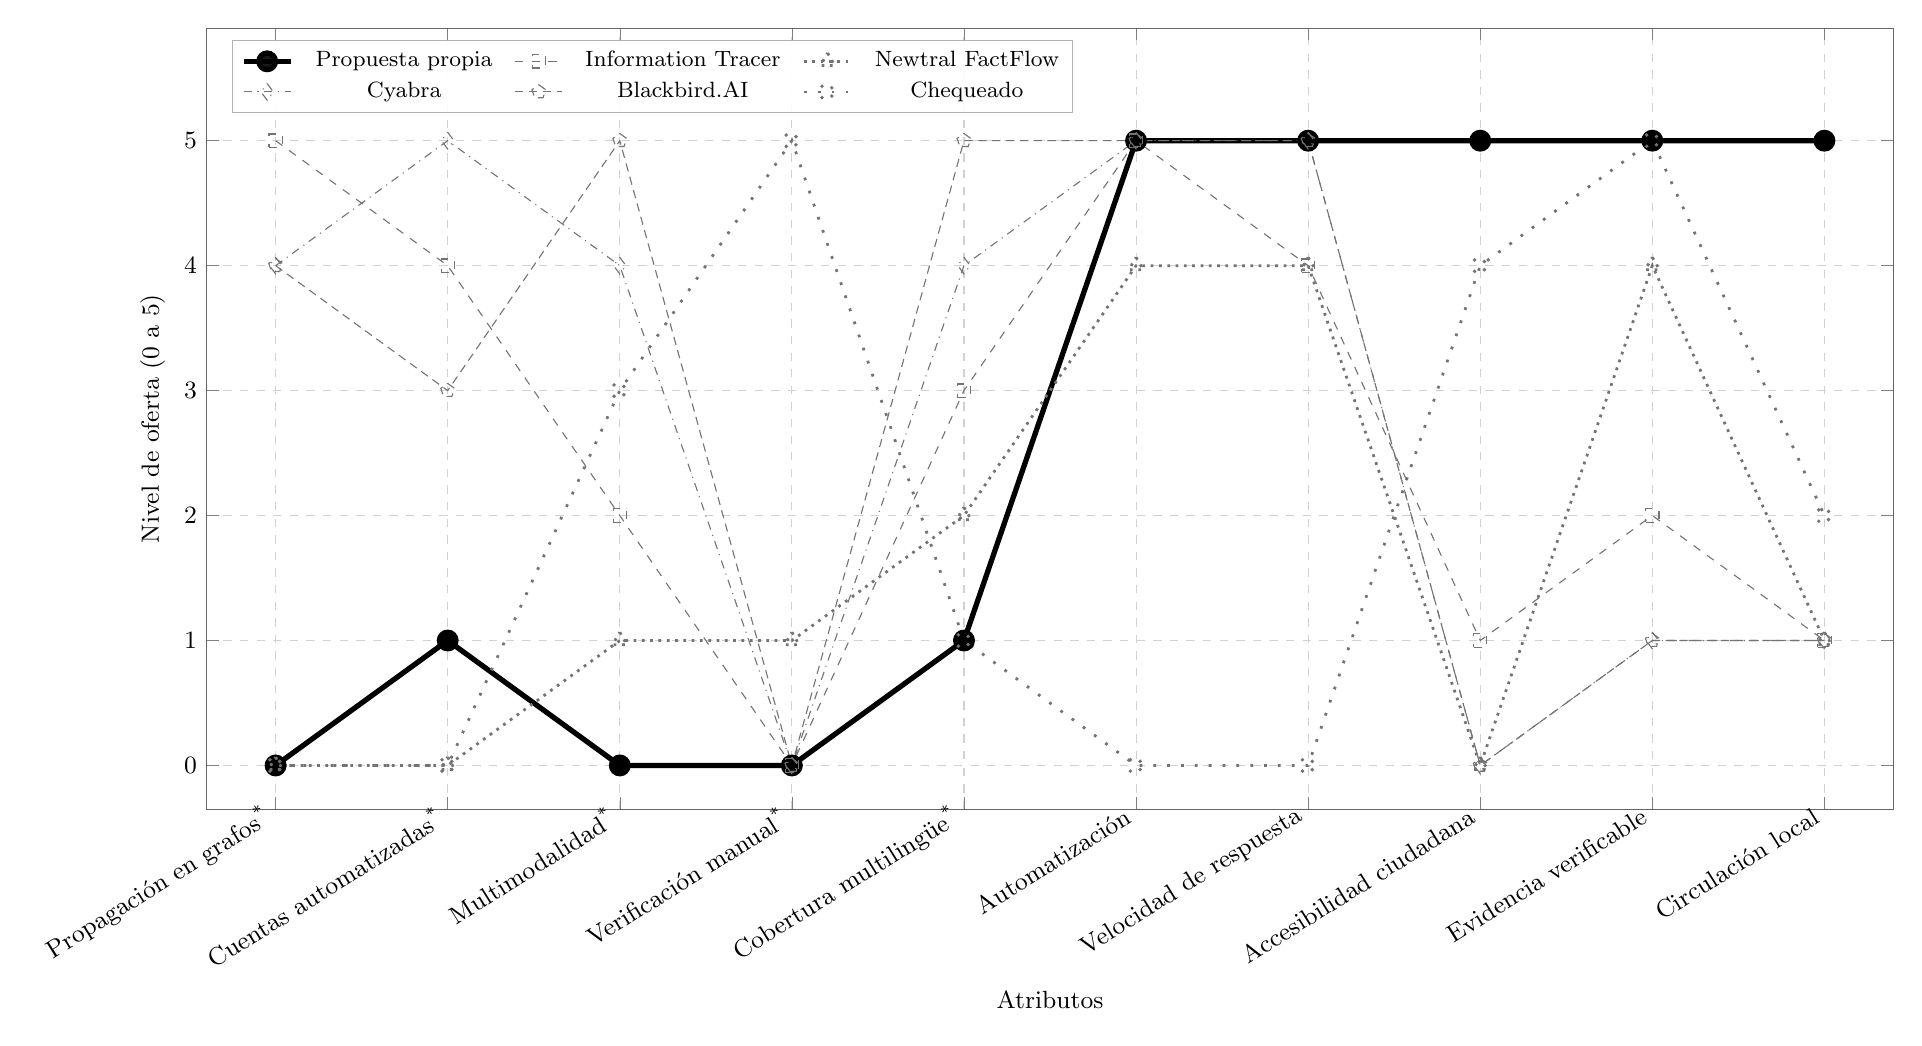
\begin{tikzpicture}
    \begin{axis}[
      width=23cm, height=11.5cm,
      ymin=-0.35, ymax=5.9,
      ytick={0,1,2,3,4,5},
      ylabel={Nivel de oferta (0 a 5)},
      xlabel={Atributos},
      xmin=0.6, xmax=10.4,
      xtick={1,2,3,4,5,6,7,8,9,10},
      xticklabels={%
        {Propagación en grafos\textsuperscript{*}},
        {Cuentas automatizadas\textsuperscript{*}},
        {Multimodalidad\textsuperscript{*}},
        {Verificación manual\textsuperscript{*}},
        {Cobertura multilingüe\textsuperscript{*}},
        {Automatización},
        {Velocidad de respuesta},
        {Accesibilidad ciudadana},
        {Evidencia verificable},
        {Circulación local}},
      x tick label style={rotate=32, anchor=east, font=\small},
      y tick label style={font=\small},
      label style={font=\small},
      legend style={at={(0.015,0.985)}, anchor=north west, font=\footnotesize,
                    legend columns=3, draw=black!30, fill=white, fill opacity=0.9,
                    text opacity=1, column sep=6pt},
      grid=major, grid style={dashed, black!18},
      axis line style={black!60},
      ]
      \addplot[line width=1.9pt, mark=*, mark size=3pt, color=black]
        coordinates {(1,0)(2,1)(3,0)(4,0)(5,1)(6,5)(7,5)(8,5)(9,5)(10,5)};
      \addlegendentry{Propuesta propia}

      \addplot[dashed, mark=square, mark size=2.4pt, color=black!55]
        coordinates {(1,5)(2,4)(3,2)(4,0)(5,3)(6,5)(7,4)(8,1)(9,2)(10,1)};
      \addlegendentry{Information Tracer}

      \addplot[dotted, line width=1pt, mark=triangle, mark size=3pt, color=black!55]
        coordinates {(1,0)(2,0)(3,1)(4,1)(5,2)(6,4)(7,4)(8,0)(9,4)(10,1)};
      \addlegendentry{Newtral FactFlow}

      \addplot[dashdotted, mark=diamond, mark size=3pt, color=black!55]
        coordinates {(1,4)(2,5)(3,4)(4,0)(5,4)(6,5)(7,5)(8,0)(9,1)(10,1)};
      \addlegendentry{Cyabra}

      \addplot[densely dashed, mark=pentagon, mark size=2.6pt, color=black!55]
        coordinates {(1,4)(2,3)(3,5)(4,0)(5,5)(6,5)(7,5)(8,0)(9,1)(10,1)};
      \addlegendentry{Blackbird.AI}

      \addplot[loosely dotted, line width=1pt, mark=x, mark size=3.4pt, color=black!55]
        coordinates {(1,0)(2,0)(3,3)(4,5)(5,1)(6,0)(7,0)(8,4)(9,5)(10,2)};
      \addlegendentry{Chequeado}
    \end{axis}
  \end{tikzpicture}
  \caption{Curva de valor de la propuesta frente a las soluciones existentes. Los atributos señalados con asterisco corresponden a capacidades cuya construcción se descartó, en las que un valor menor resulta preferible. Fuente: elaboración propia.}
  \label{fig:curva-valor}
\end{figure}
\end{landscape}

La curva evidencia que la propuesta no alcanza el nivel máximo en la totalidad de las variables, circunstancia esperable y coherente con la matriz: obtiene los valores más bajos del conjunto en las cinco primeras, que son precisamente aquellas cuya construcción se descartó, y Chequeado la iguala en evidencia verificable.

El despegue respecto de las demás soluciones se produce en un punto único: la combinación de accesibilidad para el ciudadano con automatización y velocidad de respuesta. Las cuatro soluciones automáticas obtienen valores de 0 o 1 en accesibilidad, mientras que la única accesible obtiene 0 en automatización y en velocidad. Ninguna reúne las tres condiciones, y esa intersección vacante constituye el espacio que la propuesta ocupa. La variable creada, información sobre circulación local, es la única en la que la distancia respecto del competidor más próximo alcanza los cuatro puntos, y no resulta casual que sea también la que sostiene el modelo de negocio descrito en la Sección~\ref{sec:negocio}.

\subsection{Análisis de fortalezas, oportunidades, debilidades y amenazas}

La Tabla~\ref{tab:foda} presenta el análisis FODA de la propuesta, que organiza los factores internos y externos según su incidencia positiva o negativa sobre la viabilidad del proyecto.

\begin{table}[t]
  \centering
  \small
  \caption{Análisis de fortalezas, oportunidades, debilidades y amenazas. Fuente: elaboración propia.}
  \label{tab:foda}
  \begin{tabular}{p{1.6cm} p{5.6cm} p{5.6cm}}
    \hline
    & \textbf{Positivo} & \textbf{Negativo} \\
    \hline
    \textbf{Interno} &
    \textbf{Fortalezas.} Conjunto de datos difícil de replicar sin adopción ciudadana. Foco en el español rioplatense y en fuentes argentinas. Evidencia verificable y no únicamente un veredicto. Costos operativos reducidos durante el desarrollo &
    \textbf{Debilidades.} El modelo depende íntegramente de lograr adopción. Riesgo de falsos positivos ante sátira e ironía. Equipo reducido. El clasificador requiere entrenamiento y validación continuos \\
    \textbf{Externo} &
    \textbf{Oportunidades.} Ciclos electorales recurrentes con alta demanda de monitoreo. La inteligencia artificial generativa como vector creciente de desinformación. Ausencia de competidor local con foco ciudadano. Tendencia regulatoria hacia la transparencia algorítmica &
    \textbf{Amenazas.} Regulación sobre el tratamiento de datos. Cambios en las plataformas que limiten la extracción de contenido. Competidores establecidos que se orienten al segmento ciudadano. Riesgo reputacional si el producto se percibe como sesgado \\
    \hline
  \end{tabular}
\end{table}

\section{Modelo de Negocio}
\label{sec:negocio}

\subsection{Propuesta de valor}

El sistema opera bajo un modelo de acceso gratuito con monetización orientada a organizaciones. La extensión resulta gratuita para el ciudadano, y su uso genera el activo central del negocio: un registro de qué contenido desinformativo circula en Argentina, con qué intensidad y sobre qué temas.

Corresponde precisar qué se comercializa, porque no es la extensión. Lo que se comercializa es información sobre la circulación de contenido desinformativo, y se entrega en dos formatos. El primero es una interfaz de programación de clasificación, que cualquier sistema externo puede consultar para obtener el veredicto y la evidencia sobre un texto, con precio por volumen de consultas. El segundo consiste en reportes y paneles de tendencias, que presentan qué temas circulan en un período determinado y con qué intensidad, con precio por suscripción. Ambos productos se nutren del mismo conjunto de datos, generado por el uso ciudadano de la extensión.

La lógica responde a un efecto de red de datos: cuanto mayor es la base de usuarios, más completo resulta el registro; cuanto más completo el registro, mayor el valor del producto comercial; y cuanto mayor el ingreso, mejor el producto gratuito que alimenta la base. La capa gratuita no constituye entonces una acción filantrópica ni un producto de captación, sino la fuente del dato que vuelve posible el producto pago.

Conviene delimitar el alcance de esa observación. El sistema analiza el contenido de las publicaciones que el usuario tiene a la vista en la red social; no registra qué enlaces abre, no observa otras plataformas y no alcanza a los servicios de mensajería cifrada, que en Argentina constituyen un vector de difusión relevante pero permanecen fuera del alcance del prototipo. La extensión del alcance a otras superficies constituye una línea de trabajo futura y no un supuesto del modelo.

\subsection{Segmentos de clientes}

Se identifican cinco segmentos de organizaciones con capacidad de pago y con una necesidad que el producto atiende. Los \textbf{medios de comunicación} requieren detectar tempranamente qué contenido falso circula sobre los temas que cubren. Las \textbf{organizaciones de verificación} necesitan priorizar qué afirmaciones verificar, dado que su capacidad de producción resulta acotada y la selección determina su impacto. Los \textbf{centros de investigación y observatorios} requieren series históricas para el estudio de la desinformación, insumo que hoy no existe de forma sistemática para el país. Los \textbf{organismos públicos y las organizaciones no gubernamentales} demandan monitoreo durante períodos electorales. Las \textbf{marcas y agencias de comunicación} necesitan detectar contenido falso que involucre a sus representados.

\subsection{Modelo de negocio en bloques}

La Tabla~\ref{tab:bmc} presenta el modelo mediante los nueve bloques del lienzo propuesto por Osterwalder \parencite{OsterwalderPigneur2010}.

\begin{small}
\begin{longtable}{@{}p{3.2cm} p{11cm}@{}}
  \caption{Modelo de negocio expresado en los nueve bloques del lienzo. Fuente: elaboración propia.}
  \label{tab:bmc} \\
  \hline
  \textbf{Bloque} & \textbf{Contenido} \\
  \hline
  \endfirsthead
  \hline
  \textbf{Bloque} & \textbf{Contenido} \\
  \hline
  \endhead
  \hline
  \endfoot
  Propuesta de valor & Para el ciudadano, detección automática y gratuita de contenido desinformativo con evidencia verificable durante la navegación. Para las organizaciones, información sobre la circulación de contenido desinformativo en el país, accesible mediante interfaz de programación y reportes \\
  Segmentos de clientes & Ciudadanos argentinos que consumen noticias en la red social, con un segmento primario de validación de 18 a 40 años interesado en política y economía. Organizaciones: medios, verificadores, centros de investigación, organismos públicos y agencias de comunicación \\
  Canales & Para el ciudadano, la tienda de extensiones del navegador, el sitio del producto y la difusión en prensa y redes. Para las organizaciones, venta directa, sitio institucional y alianzas con asociaciones profesionales del sector \\
  Relación con los clientes & Autogestión y soporte por correo para el ciudadano. Suscripción autogestionada para organizaciones pequeñas. Contrato anual con acuerdo de nivel de servicio para organizaciones de mayor porte \\
  Fuentes de ingreso & Consultas a la interfaz de programación con precio escalonado por volumen. Suscripción mensual a reportes y paneles. Contratos anuales. Contratos puntuales de monitoreo electoral \\
  Recursos clave & El conjunto de datos sobre circulación de contenido desinformativo en el país; el clasificador adaptado al español rioplatense; la base de usuarios que alimenta ese conjunto; y la reputación de imparcialidad \\
  Actividades clave & Mantenimiento y mejora del clasificador. Mantenimiento de la extensión y del servicio. Elaboración de reportes. Venta a organizaciones. Comunicación con la base de usuarios. Cumplimiento normativo \\
  Socios clave & Organizaciones de verificación, en calidad de posibles clientes y socios académicos y no como fuente de datos, dado que el sistema no accede de forma automatizada a sus sitios. Medios de referencia como fuente de evidencia. Proveedores de inferencia y de búsqueda. Universidades para investigación y validación \\
  Estructura de costos & Infraestructura de servicio y base de datos, alojamiento del panel, servicio de inferencia y servicio de búsqueda. Venta y comunicación. Desarrollo y mantenimiento. Cumplimiento normativo. Los costos crecen con el volumen, con mejora del margen a escala \\
\end{longtable}
\end{small}

\subsection{Análisis de las cinco fuerzas competitivas}

El análisis de las fuerzas que determinan la rentabilidad de un sector \parencite{Porter2008} arroja el siguiente cuadro para la propuesta.

La \textbf{rivalidad entre los competidores existentes} resulta moderada. Las plataformas comerciales relevadas operan sobre segmentos distintos, organismos gubernamentales y redacciones de gran porte, de modo que en el segmento ciudadano local no se registra competencia directa.

El \textbf{poder de negociación de los clientes} resulta elevado en la etapa inicial, dado que existen alternativas y la propuesta carece de trayectoria, y decrece a medida que el conjunto de datos se vuelve difícil de sustituir. Su mitigación consiste en contratos anuales y en una integración profunda con los procesos del cliente.

El \textbf{poder de negociación de los proveedores} resulta moderado. La propuesta depende de la tienda de extensiones del navegador, del servicio de inferencia y del servicio de búsqueda, con el consiguiente riesgo de cambios en sus precios o en sus políticas. Su mitigación consiste en una arquitectura modular que permita sustituir cada servicio, criterio que la Sección~\ref{sec:arquitectura} incorpora de forma explícita.

La \textbf{amenaza de nuevos participantes} resulta de moderada a baja. La barrera técnica es reducida, puesto que los modelos se encuentran disponibles de forma abierta, pero la barrera de datos es elevada y se incrementa con el tiempo por efecto de la red de datos descrita.

La \textbf{amenaza de productos sustitutos} resulta elevada y constituye la fuerza más significativa del cuadro. Operan como sustitutos la verificación manual, la búsqueda por cuenta propia del usuario y los mecanismos de anotación colaborativa que las propias plataformas incorporan. El sustituto de mayor peso a futuro consiste en que las plataformas integren detección nativa. Su mitigación se apoya en el foco local, en la evidencia verificable y en la independencia respecto de la plataforma analizada.

\subsection{Estructura de precios}

La Tabla~\ref{tab:pricing} presenta la estructura de precios prevista. Los valores son tentativos y su ajuste requiere validación de mercado, que no forma parte del alcance del presente trabajo.

\begin{table}[t]
  \centering
  \small
  \caption{Estructura de precios prevista por producto y segmento. Fuente: elaboración propia.}
  \label{tab:pricing}
  \begin{tabular}{p{4.4cm} p{4.2cm} p{4.6cm}}
    \hline
    \textbf{Producto} & \textbf{Segmento} & \textbf{Precio tentativo} \\
    \hline
    Extensión de navegador & Ciudadano & Gratuito \\
    Interfaz de programación, nivel inicial & Desarrollo y evaluación & 1.000 consultas mensuales sin cargo \\
    Interfaz de programación, nivel intermedio & Medios pequeños y verificadores & USD 200 mensuales por 50.000 consultas \\
    Interfaz de programación, nivel superior & Medios de gran porte y marcas & USD 1.500 a 5.000 mensuales, con acuerdo de nivel de servicio \\
    Panel de tendencias & Verificadores y observatorios & USD 300 mensuales \\
    Reportes de monitoreo electoral & Organismos públicos y organizaciones no gubernamentales & USD 10.000 a 50.000 por contrato de tres a seis meses \\
    Acceso histórico al conjunto de datos & Universidades e investigación & USD 100 mensuales por suscripción institucional \\
    \hline
  \end{tabular}
\end{table}

\subsection{Mezcla de marketing}

La mezcla de marketing organiza en cuatro dimensiones las decisiones comerciales que las secciones anteriores desarrollan por separado. Se presenta de forma tentativa, en el mismo carácter que la estructura de precios, dado que su validación depende de la investigación con usuarios y del contacto con las organizaciones destinatarias.

\textbf{Producto.} La oferta se compone de cuatro elementos con destinatarios diferenciados. La extensión de navegador constituye el producto orientado al ciudadano y se ofrece sin costo; su diseño se describe en la Sección~\ref{sec:interfaz}. La interfaz de programación de detección permite a una organización incorporar el análisis en sus propios procesos. El panel de tendencias entrega la información agregada sobre circulación de contenido desinformativo. Los informes por período o por evento constituyen el formato de mayor elaboración, orientado a organismos públicos y organizaciones de la sociedad civil durante ciclos de alta circulación.

\textbf{Precio.} La estructura tarifaria se detalla en la Tabla~\ref{tab:pricing} y responde a un modelo escalonado por volumen de consultas. La decisión que la gobierna requiere una precisión: la gratuidad del producto ciudadano no constituye una acción promocional ni un período de prueba, sino el mecanismo que produce el activo que se comercializa. Cada publicación analizada por un usuario sin costo incrementa el registro de circulación que sostiene el producto pago, de modo que el segmento gratuito no representa un costo de adquisición sino la fuente de suministro.

\textbf{Plaza.} La distribución opera por dos canales según el destinatario. El producto ciudadano se distribuye a través de la tienda de extensiones del navegador, que concentra el descubrimiento y resuelve la instalación y la actualización sin intervención del usuario. La oferta orientada a organizaciones se comercializa mediante venta directa, apoyada en un sitio institucional y en acuerdos con asociaciones profesionales del sector periodístico y con organizaciones de verificación, que operan como vía de acceso a los segmentos descritos.

\textbf{Promoción.} La difusión se apoya en tres líneas. La primera consiste en el lanzamiento a través de socios institucionales, dado que la recomendación proveniente de una organización de verificación o de un medio reconocido aporta la credibilidad que un producto sobre veracidad no puede reclamar por sí mismo. La segunda concentra la comunicación en los ciclos electorales y en episodios de alta circulación de contenido desinformativo, períodos en los que la disposición del público a incorporar una herramienta de este tipo resulta considerablemente mayor. La tercera es la presencia académica: la publicación del trabajo y, en su momento, del corpus disociado, opera simultáneamente como contribución de investigación y como vía de difusión hacia el ámbito universitario y los observatorios, que integran uno de los segmentos identificados.

Corresponde señalar que la matriz de crecimiento y participación no se incorpora al análisis. Su aplicación requiere una cartera de productos entre los cuales distribuir la inversión, condición que no se verifica en una propuesta de producto único.

\subsection{Misión y visión}

La \textbf{misión} consiste en poner a disposición de cualquier ciudadano argentino una herramienta automática y verificable que le permita identificar contenido desinformativo mientras consume información digital, y construir sobre esa base un registro sistemático de la circulación de desinformación en el país.

La \textbf{visión} consiste en constituirse en la referencia del ecosistema informativo argentino sobre esa materia: la fuente que medios, verificadores, investigadores y organismos públicos consultan cuando necesitan conocer qué contenido desinformativo circula, con qué intensidad y sobre qué temas.

\subsection{Riesgos del modelo}

Cuatro riesgos condicionan la viabilidad del modelo y admiten mitigaciones de distinto alcance.

El \textbf{riesgo de adopción} es el de mayor peso, dado que la totalidad del modelo depende de alcanzar una base de usuarios significativa: sin usuarios no existe conjunto de datos, y sin conjunto de datos el producto comercial pierde su diferencial. Su mitigación consiste en una estrategia de lanzamiento apoyada en socios institucionales y en la comunicación durante los ciclos electorales.

El \textbf{riesgo regulatorio} se vincula con la normativa sobre protección de datos personales y con eventuales regulaciones sobre el monitoreo de redes sociales. Su mitigación se desarrolla en la Sección~\ref{sec:legal} y se incorpora al diseño mediante la anonimización de toda entrega hacia terceros y la ausencia de tratamiento de datos personales del usuario.

El \textbf{riesgo reputacional} deriva de que un producto que clasifica contenido como sospechoso puede percibirse como políticamente sesgado. Su mitigación consiste en la presentación de evidencia verificable en lugar de veredictos sin justificación, criterio que RNF-06 y RNF-07 incorporan como requerimiento y no como intención.

El \textbf{riesgo competitivo} consiste en que una plataforma establecida lance una extensión gratuita y replique la estrategia. Su mitigación se apoya en la ventaja de anticipación, en el foco local y en el efecto de red de datos, que se acentúa con el transcurso del tiempo.
